  
\documentclass[12pt,a4paper,fleqn]{tufte-handout} 
\usepackage{graphicx} 
\usepackage{morefloats} 
\usepackage{amsmath} 
\usepackage{amssymb} 
\usepackage{rotating} 
% mcode options for matlab code insertion bw (for printing), numbered (line numbers), framed (frame around code blocks), useliterate (convert Matlab expressions to Latex ones), autolinebreaks (automatic code wraping, use it with caution 
\usepackage[literate]{mcode} 
\graphicspath{{figures/}{tex/}{../figures/}{../../}{../}}  
\title{distanceDemonstration} 
\author{ Mathieu Lagrange } 
  
\begin{document} 
  
\maketitle 
  
% Please use this file to document your experiment 
% You can compile the report by setting the option 'report' as detailed in your expCode configuration file. 

\section{Introduction}

This document documents the first demonstration of the use of the expCode framework to conduct a computational experiment. The project distanceDemonstration is about the comparison of several distances over synthetic data.



\section{Design}

 The project is divided into two processing steps:
\begin{enumerate}
\item \textbf{generate}: generation of the synthetic datasets
\item \textbf{compute}: computation of the distances over those datasets and performance metrics
\end{enumerate}

\subsection{\textbf{Generate step}: generation of synthetic datasets}

Each dataset comprises a set of points in a space of given dimensionality. Those points are grouped into classes whose centroid are spread along the diagonal. The degree of overlap between classes is controlled by the spread of the points with respect to the centroid of its class. The needed factors of variability that are to be tested are:
\begin{enumerate}
\item the number of classes
\item the dimensionality of the space
\item the spread of the data points of a given class
\item the number of replications
\item the number of data points per class.
\end{enumerate}

\begin{marginfigure}
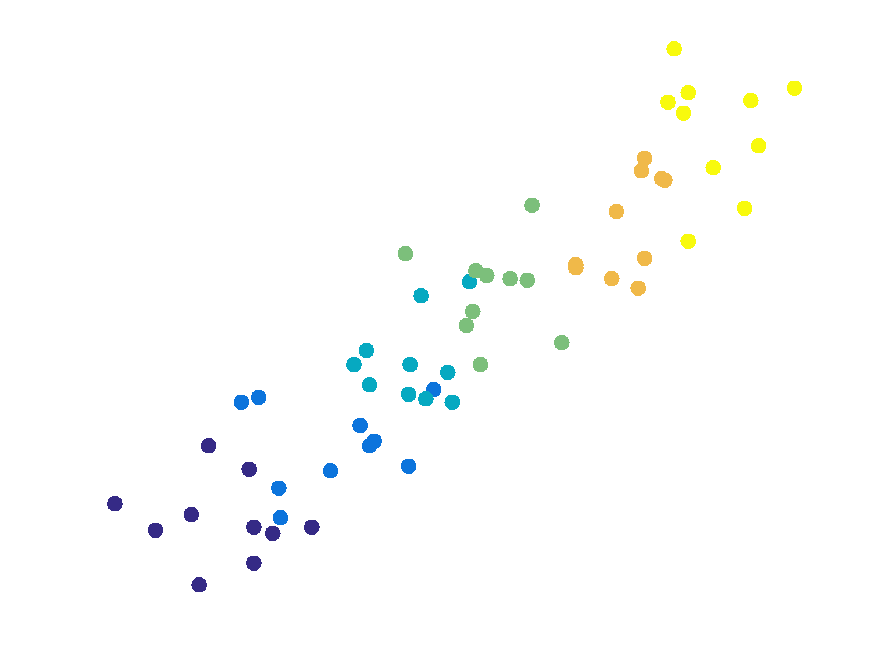
\includegraphics[width=\textwidth]{figures/scatter}
\caption{A dataset with average spread.}
\label{scatter}
\end{marginfigure}

This step outputs for each dataset the location of the data points (elements) as well as the class to which they belong to (class).

\subsection{\textbf{Compute step}: Computation of distances}

Once the datasets are generated, we can compute the distances between all points of a given dataset. The factor for this step is then:
\begin{enumerate}
\item the type of distances.
\end{enumerate}

We consider three distance, the well-known Euclidean distance, with or without prior standardization over the dimensions of the space, and the cosine distance defined as:
$$
d_c(x, y) = 1-\frac{xy'}{\sqrt{(xx')(yy')}}
$$

\subsection{Observations}

Since we consider distances between data points that each belong to a given class, ranking metrics are appropriate to evaluate the performance of those distances on the generated datasets \cite{manning2008introduction}. More precisely, we consider the following metrics:
\begin{enumerate}
\item map: mean average precision
\item precision: precision at rank 5.
\end{enumerate}

\section{Definition of factors}

Those factors and their corresponding modalities are defined in the file named \texttt{dideFactors.txt} whose content is the following:
\lstinputlisting{../dideFactors.txt}

Please note the 2 between the first two equals of the factor definition of factor \textit{distance} which specify that this factor is needed only for the second processing step. Most the factor design diccused above is compactly displayed in Figure \ref{factorFlowGraph}. Modalities\texttt{nbRealizations} and \texttt{nbElementsPerClass} are fixed .

\begin{figure}
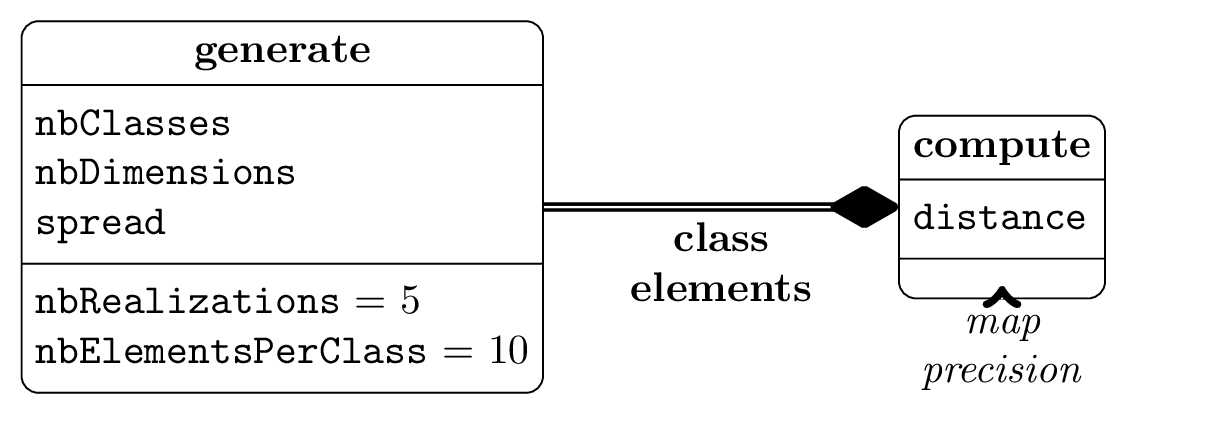
\includegraphics[width=\textwidth]{figures/factors}
\caption{A dataset with maximal spread.}
\label{scatter}
\end{figure}

\section{Implementation}

Each processing step his implemented in a given file.

\subsection{Step 1: generate}

The datasets are generated with the following code:
\lstinputlisting[firstline=20, lastline=26]{../dide1generate.m}

\subsection{Step 2: compute} 


The data points are retrieved and, for some distances, pre-processed as follows:
\lstinputlisting[firstline=20, lastline=26]{../dide2compute.m} 

Then, the actual distances are computed as follows:
\lstinputlisting[firstline=27, lastline=37]{../dide2compute.m} 
Since the complete distance matrix is symmetric, only half the values are computed.

The observations, namely the 2 metrics  are generated and stored as follows:
  \lstinputlisting[firstline=38, lastline=40]{../dide2compute.m} 

\section{Results}

This report and all needed data can be generated using the following command:

 \mcode{distanceDemonstration('do', 0, 'report', 'rccv');}

\subsection{Morphology of the datasets}

We first want to study three factors that influence the performance of the different ranking metrics, namely the number of classes, the number of dimensions of the space and the intra class spread. To this matter, we set the metric to be the well known euclidean distance. Table \ref{nbdi5Sp60Dieu} shows the impact of the number of classes. As the number of classes increases, the problem appears to become harder even though no statistical difference can be found.

Table \ref{nbcl6Sp60Dieu} shows the impact of the number of dimensions. As this factor increases, the separability grows and consequently lead to a significant increase in performance.

Figure \ref{nbcl6Nbdi5Dieu} shows the negative impact of the intra class spread on the MAP.

Those three displays are respectively generated by the following lines:
\lstinputlisting[firstline=11, lastline=13]{../dideReport.m}

\subsection{Distance Metrics}

We chose to study three distances, respectively the Euclidean distance, the standardization Euclidean distance and the cosine distance. Given the morphology of the datasets, the standardization shall have a negligible impact on the performance. This is numerically verified by the experiment as shown on Table \ref{nbcl6Nbdi5Sp60}, where no statistical  can be found over those two distances. 

Considering the cosine distance have a significant negative impact on the performance, as the implied magnitude normalization is not meaningful for the datasets considered.
  
\input{tex/exposeTmp} % expCodeInsertionFlag DO NOT CLEAR (but move it where you want the generated temporary LaTEX code to be inserted) 
  
  
\bibliographystyle{abbrvnat} 
\bibliography{bib} 
  
\end{document} 
